\section{Libreoffice \emph{online}}

Au sein du nuage, \emph{LibreOffice OnLine\/} ou encore LOOL a été intégrée, toujours dans le menu $\oplus$ et offre le traitement de textes \emph{writer\/}, le tableur \emph{calc\/} et le logiciel de présentation \emph{impress\/}, permettant d'ouvrir les document montés sur le nuage mais aussi d'éditer ceux déjà présents.

Ainsi vous accéderez aux trois outils de la suite bureautique libreoffice online les plus utilisés, le traitement de textes \emph{writer\/}, le tableur \emph{calc\/} et le logiciel de présentations \emph{impress\/} comme le montrent les captures suivantes.

\begin{figure}
    \centering
    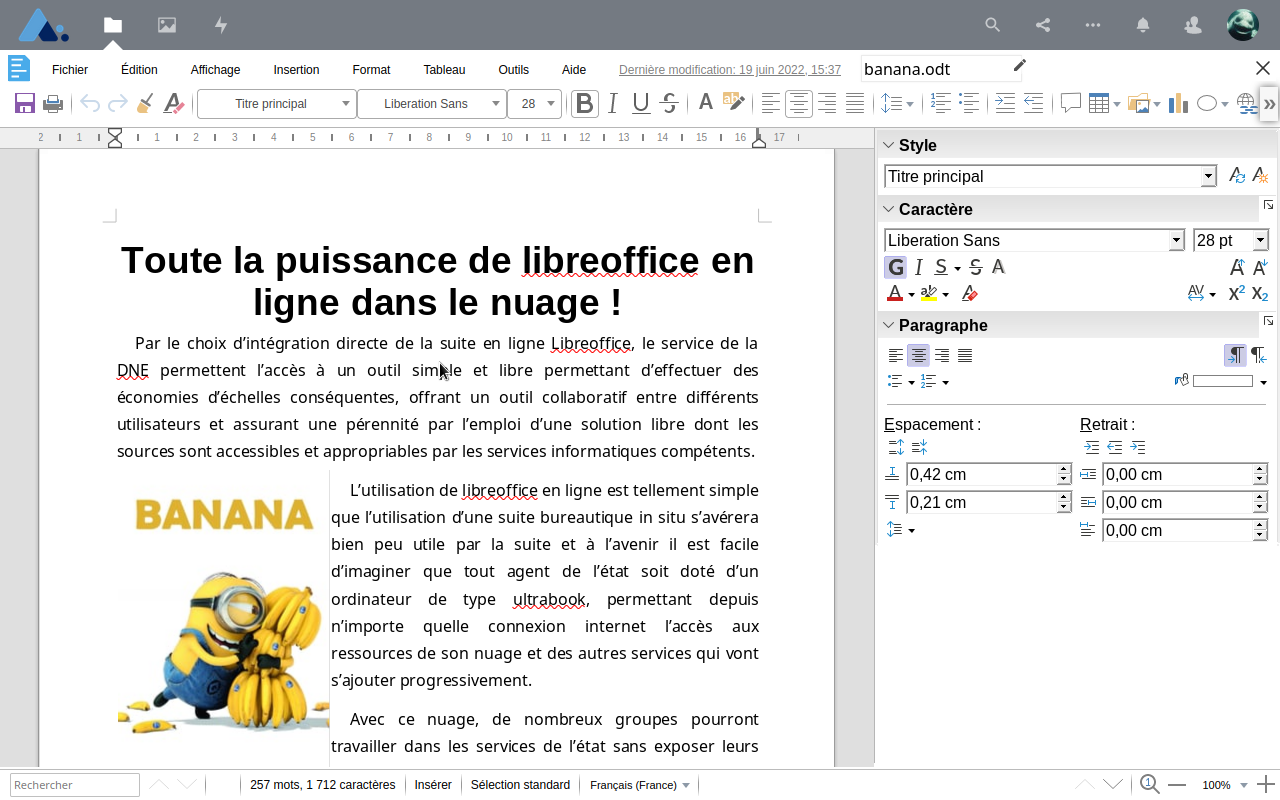
\includegraphics[]{Captures/nuage.lool.writer.png}
    \caption{Exemple de fichier de traitement de textes composé dans Libreoffice \emph{writer\/} au sein du nuage.}
\end{figure}

La capture d'écran ci-avant montre un document rédigé entièrement en ligne, inclusion d'image comprise, avec le volet latéral de Libreoffice actif.

Il faut prendre en compte quelques points néanmoins, l'un d'entre eux est qu'à l'instar de la suite \emph{Office\/} de Microsoft\textregistered{} la version en ligne n'est pas complète mais une version allégée. 
Les utilisateurs avancés de Libreoffice se verront amputés de quelques fonctionnalités, par exemple en ce qui me concerne, l'éditeur d'équations.
Notez cependant qu'un fichier édité en local, \emph{i.e.\/} sur un ordinateur directement par la version complète de Libreoffice sera conservé lors du transfert, et, s'il y a ouverture, sera considéré comme un objet inséré dans le document malgré l'impossibilité d'éditer directement son contenu.

\begin{figure}
    \centering
    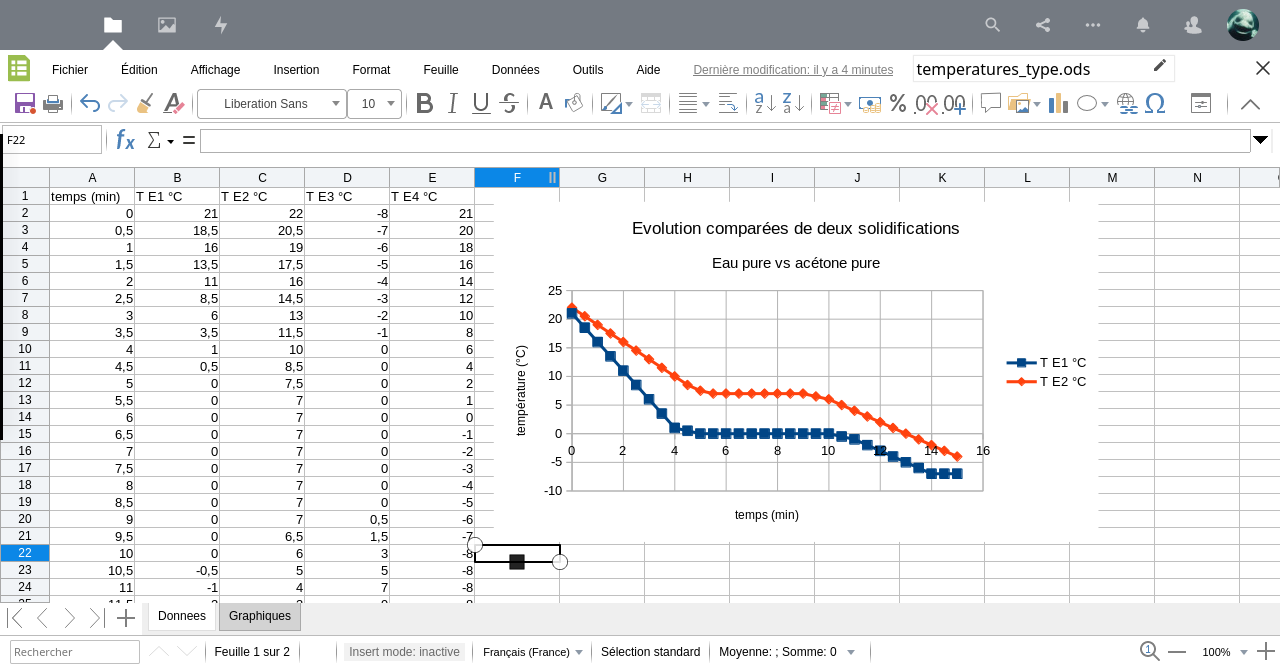
\includegraphics[]{Captures/nuage.lool.tableur.png}
    \caption{Un exemple de tableur/grapheur sous Libreoffice \emph{Calc\/} et un graphique inséré, le tout directement en ligne.}
\end{figure}

Le tableur permet l'édition de formules et l'insertion de graphiques, comme on pouvait l'espérer.

\begin{figure}
    \centering
    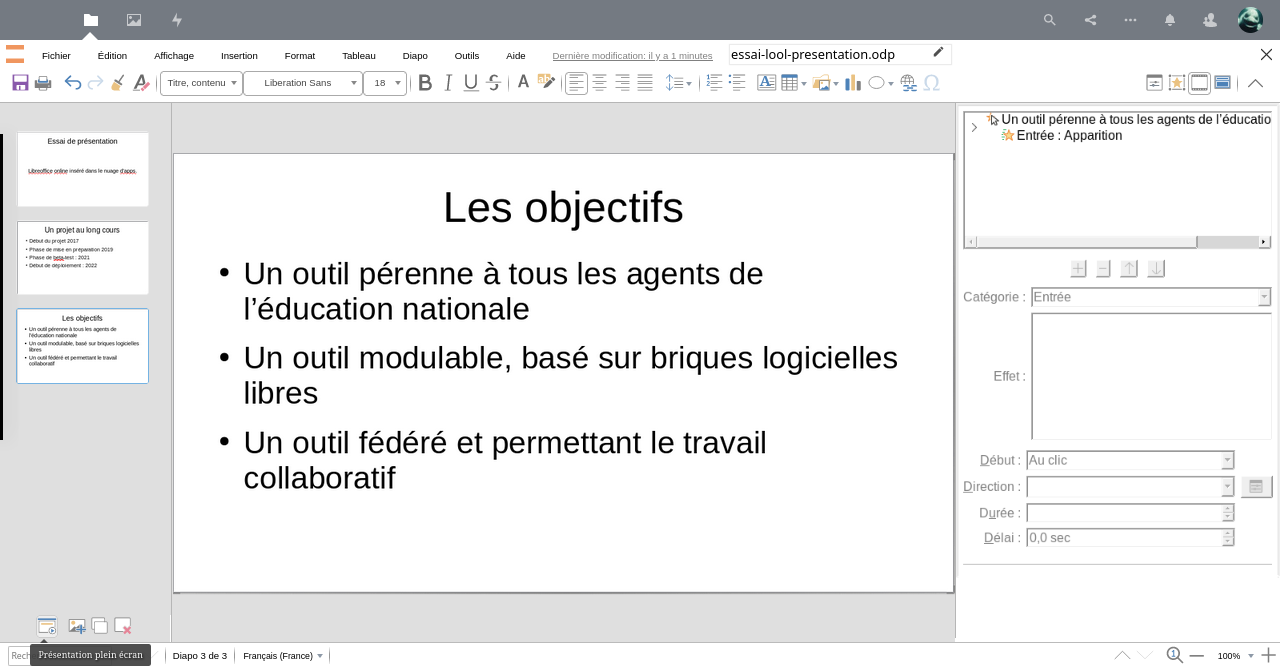
\includegraphics[]{Captures/nuage.lool.presentation.png}
    \caption{Une ébauche de présentation de Libreoffice \emph{Impress\/} en plein développement.}
\end{figure}

Et évidemment il est possible de créer des présentations simples voire complexes le tout en ligne, ou de les modifier.

La suite bureautique Libreoffice Online permet aussi d'exporter, et \emph{de facto} de télécharger les documents produits dans divers formats, l'exemple suivant montre les exportations associées à \emph{Writer\/}.

\begin{figure}
    \centering
    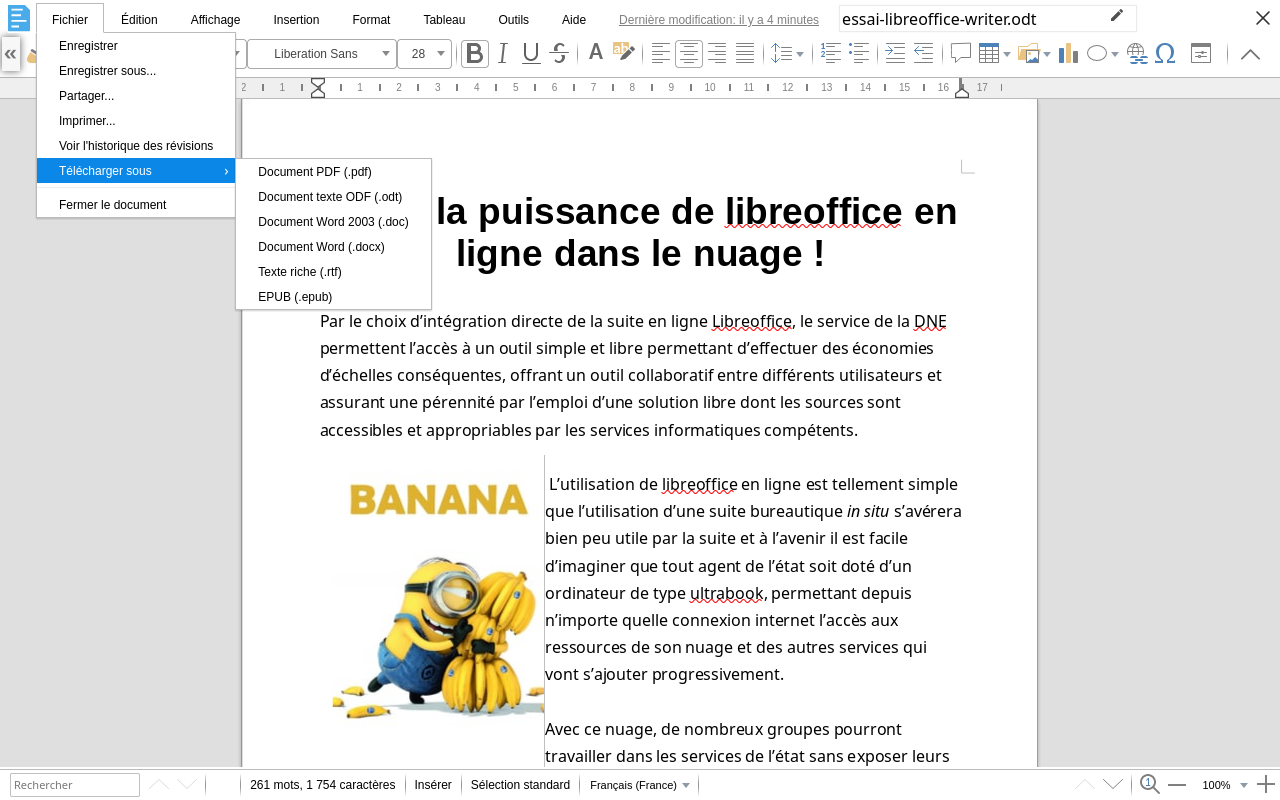
\includegraphics[]{Captures/nuage.lool.writer.exportations.png}
    \caption{Les exportations proposées dans Libreoffice \emph{writer\/}.}
\end{figure}

Cette fois-ci vous aurez noté que le volet latéral est occulté.